\documentclass[11pt]{article}
\usepackage[margin=1in]{geometry}
\usepackage{amsmath}
\usepackage{amssymb}
\usepackage{booktabs}
\usepackage{graphicx}
\usepackage{float}
\usepackage{hyperref}
\usepackage{setspace}
\usepackage{titlesec}
\usepackage{caption}
\usepackage{microtype}
\usepackage{array}
\usepackage{tabularx}
\usepackage{enumitem}
\usepackage{fancyhdr}
\usepackage{abstract}
\hypersetup{colorlinks=true, linkcolor=black, urlcolor=blue, citecolor=black}
\setstretch{1.12}
\setlength{\parindent}{0pt}
\setlength{\parskip}{0.55em}
\captionsetup{font=small, labelfont=bf}
\titleformat{\section}{\large\bfseries}{\thesection.}{0.5em}{}
\titleformat{\subsection}{\normalsize\bfseries}{\thesubsection.}{0.5em}{}
\titlespacing*{\section}{0pt}{1.4em}{0.6em}
\titlespacing*{\subsection}{0pt}{1.0em}{0.4em}
\pagestyle{fancy}
\fancyhf{}
\lhead{IEOR 198 Final Project}
\rhead{Enhanced Volatility-Managed Allocation}
\cfoot{\thepage}
\renewcommand{\headrulewidth}{0.4pt}
\renewcommand{\footrulewidth}{0pt}
\renewcommand{\abstractnamefont}{\normalfont\bfseries}
\renewcommand{\abstracttextfont}{\normalfont\small}

\title{Enhanced Volatility-Managed Allocation with GARCH, CVaR, and a Gold Defensive Sleeve}
\author{
Chun-Kai Hsu \\
\normalsize Student ID: 3040748636 \\
\normalsize M.A. Statistics \\
\normalsize IEOR 198: Introduction to Quantitative Finance \\
\normalsize University of California, Berkeley
}
\date{Spring 2026}

\begin{document}
\maketitle
\thispagestyle{fancy}

\begin{abstract}
This project studies whether a volatility-managed, tail-risk-aware allocation strategy can improve upon a traditional stock-bond portfolio. Starting from an original proposal that dynamically allocated between SPY and TLT using GARCH volatility forecasts and Conditional Value-at-Risk (CVaR), I extend the model by adding GLD as a third defensive asset. The motivation is that the original stock-bond framework is vulnerable when equities and long-duration Treasuries fall together, as in the 2022--2024 rate-hike regime. The enhanced strategy uses a monthly walk-forward backtest from January 2008 to December 2024 and chooses portfolio weights by balancing expected return, forecast volatility, CVaR, and turnover. The main result is that the enhanced SPY/TLT/GLD strategy improves the Sharpe ratio from 0.889 in the original dynamic model to 0.991, while also reducing maximum drawdown and tail risk. This makes the extension both financially intuitive and empirically effective.
\end{abstract}

\section{Introduction}
Portfolio allocation is one of the core problems in quantitative finance. A static allocation such as 60/40 is simple and widely used, but it does not adapt to changing market conditions. A more dynamic framework can potentially improve robustness by adjusting exposure when risk rises and by reallocating toward assets with more favorable tail-risk profiles.

My original project idea focused on a dynamic SPY/TLT allocator:
\begin{itemize}
    \item forecast asset volatility using GARCH(1,1)
    \item estimate downside risk using CVaR
    \item rebalance monthly using a walk-forward process
\end{itemize}

That idea is sensible, but it has an important structural weakness. In an inflationary or rate-hike regime, long-duration bonds may no longer act as a reliable hedge. This is exactly what happened in 2022. As a result, I upgraded the project by adding GLD as a third asset. Gold provides a different risk profile from long-duration Treasuries and can act as a more diversified defensive sleeve when the stock-bond relationship breaks down.

The final research question becomes:

\begin{quote}
Can an enhanced volatility-managed allocation strategy across SPY, TLT, and GLD deliver a better risk-adjusted profile than the original SPY/TLT dynamic model and classic benchmark portfolios?
\end{quote}

\section{Dataset}
\begin{itemize}
    \item SPY: U.S. equity market exposure
    \item TLT: long-duration U.S. Treasury exposure
    \item GLD: gold exposure as an alternative defensive asset
    \item Frequency: daily adjusted close prices
    \item Source: Yahoo Finance via \texttt{yfinance}
    \item Sample: 2008-01-01 to 2024-12-31
\end{itemize}

This sample includes multiple important market regimes:
\begin{itemize}
    \item post-Global Financial Crisis recovery
    \item COVID-19 shock
    \item inflation and rate-hike regime from 2022 onward
\end{itemize}

Daily log returns are computed as
\[
r_t = \log\left(\frac{P_t}{P_{t-1}}\right).
\]

\section{Methodology}
\subsection{Walk-forward backtest}
The strategy rebalances monthly. At each rebalance date, it only uses the trailing 756 trading days of data, which is roughly three years. This produces a true out-of-sample rolling backtest rather than an in-sample fit.

\subsection{Volatility forecasting}
For each asset, I estimate a univariate GARCH(1,1) model:
\[
\sigma_t^2 = \omega + \alpha \epsilon_{t-1}^2 + \beta \sigma_{t-1}^2.
\]

This yields a one-month-ahead forecast volatility for each asset. If the optimizer fails numerically, the implementation falls back to an EWMA estimate for stability.

\subsection{Tail-risk-aware portfolio construction}
To estimate downside risk, I build rolling 21-trading-day return scenarios, which approximate one-month holding-period returns. These scenarios are volatility-scaled using the forecast-to-historical volatility ratio so that the scenario distribution reflects current market conditions.

Expected monthly returns are estimated using a blended momentum signal:
\begin{itemize}
    \item 60\% weight on trailing 6-month average returns
    \item 40\% weight on trailing 12-month average returns
\end{itemize}

The optimizer then chooses the monthly portfolio weights that maximize
\[
\text{score}(w)=\mathbb{E}[R_p(w)]-\lambda \cdot \text{CVaR}_{95\%}(w)-\kappa \cdot \text{Turnover}(w),
\]
where \(\mathbb{E}[R_p(w)]\) is the expected portfolio return, \(\text{CVaR}_{95\%}(w)\) penalizes tail losses, and Turnover discourages excessive rebalancing. For realism, the SPY weight is constrained between 10\% and 90\%.

\subsection{Why adding GLD is the key improvement}
The original SPY/TLT strategy assumes Treasuries remain a reliable hedge. That assumption is fragile. Gold introduces a distinct macro exposure and makes the model less dependent on one defensive asset. This is the main enhancement in the final version of the project and serves as the project's own twist beyond the initial proposal.

\section{Benchmarks}
I compare the final strategy against:
\begin{itemize}
    \item Original dynamic SPY/TLT
    \item Enhanced dynamic SPY/TLT/GLD
    \item Static 60/40
    \item Equal weight 1/3 across SPY, TLT, and GLD
    \item Buy-and-hold SPY
\end{itemize}

All rebalanced strategies include transaction costs of 10 bps per unit of turnover.

\section{Results}
\subsection{Full-sample performance}
\begin{table}[H]
\centering
\caption{Full-sample performance comparison}
\small
\begin{tabular}{>{\raggedright\arraybackslash}p{4.3cm}rrrrrr}
\toprule
Strategy & Cum. Ret. & Ann. Ret. & Ann. Vol. & Sharpe & Max DD & CVaR 95\% \\
\midrule
Original Dynamic SPY/TLT & 2.1825 & 0.0862 & 0.0970 & 0.8891 & -0.2827 & 0.0570 \\
Enhanced Dynamic SPY/TLT/GLD & 2.3750 & 0.0908 & 0.0916 & 0.9913 & -0.2267 & 0.0463 \\
Static 60/40 & 2.5348 & 0.0944 & 0.1005 & 0.9392 & -0.2623 & 0.0599 \\
Equal Weight 1/3 & 1.6332 & 0.0716 & 0.0945 & 0.7581 & -0.2124 & 0.0492 \\
Buy and Hold SPY & 5.0217 & 0.1368 & 0.1424 & 0.9607 & -0.2393 & 0.0841 \\
\bottomrule
\end{tabular}
\end{table}

The enhancement produces a clear improvement over the original dynamic model:
\begin{itemize}
    \item annualized return rises from 8.62\% to 9.08\%
    \item annualized volatility falls from 9.70\% to 9.16\%
    \item Sharpe ratio increases from 0.889 to 0.991
    \item maximum drawdown improves from -28.27\% to -22.67\%
    \item monthly CVaR 95\% improves from 5.70\% to 4.63\%
\end{itemize}

This is a meaningful upgrade, not just a cosmetic tweak. The improved strategy now has the best Sharpe ratio among all tested portfolios, including the static 60/40 benchmark.

\subsection{Regime analysis for the enhanced strategy}
\begin{table}[H]
\centering
\caption{Enhanced strategy regime analysis}
\small
\begin{tabular}{>{\raggedright\arraybackslash}p{4.3cm}rrrrrr}
\toprule
Regime & Cum. Ret. & Ann. Ret. & Ann. Vol. & Sharpe & Max DD & CVaR 95\% \\
\midrule
GFC Recovery to Pre-COVID & 1.5442 & 0.1093 & 0.0776 & 1.4097 & -0.0793 & 0.0332 \\
COVID Shock & 0.1130 & 0.1130 & 0.1017 & 1.1121 & -0.0731 & 0.0224 \\
Rate Hike Regime & 0.1339 & 0.0428 & 0.1221 & 0.3504 & -0.1884 & 0.0517 \\
\bottomrule
\end{tabular}
\end{table}

The regime breakdown shows why the enhancement matters. The strategy remains strong in the post-crisis and COVID periods, but the most important difference appears in the 2022--2024 rate-hike regime. The original stock-bond formulation struggled because both risky assets and the bond hedge came under pressure. Adding gold does not eliminate this challenge, but it materially improves the portfolio's resilience.

\subsection{Figures}
\begin{figure}[H]
\centering
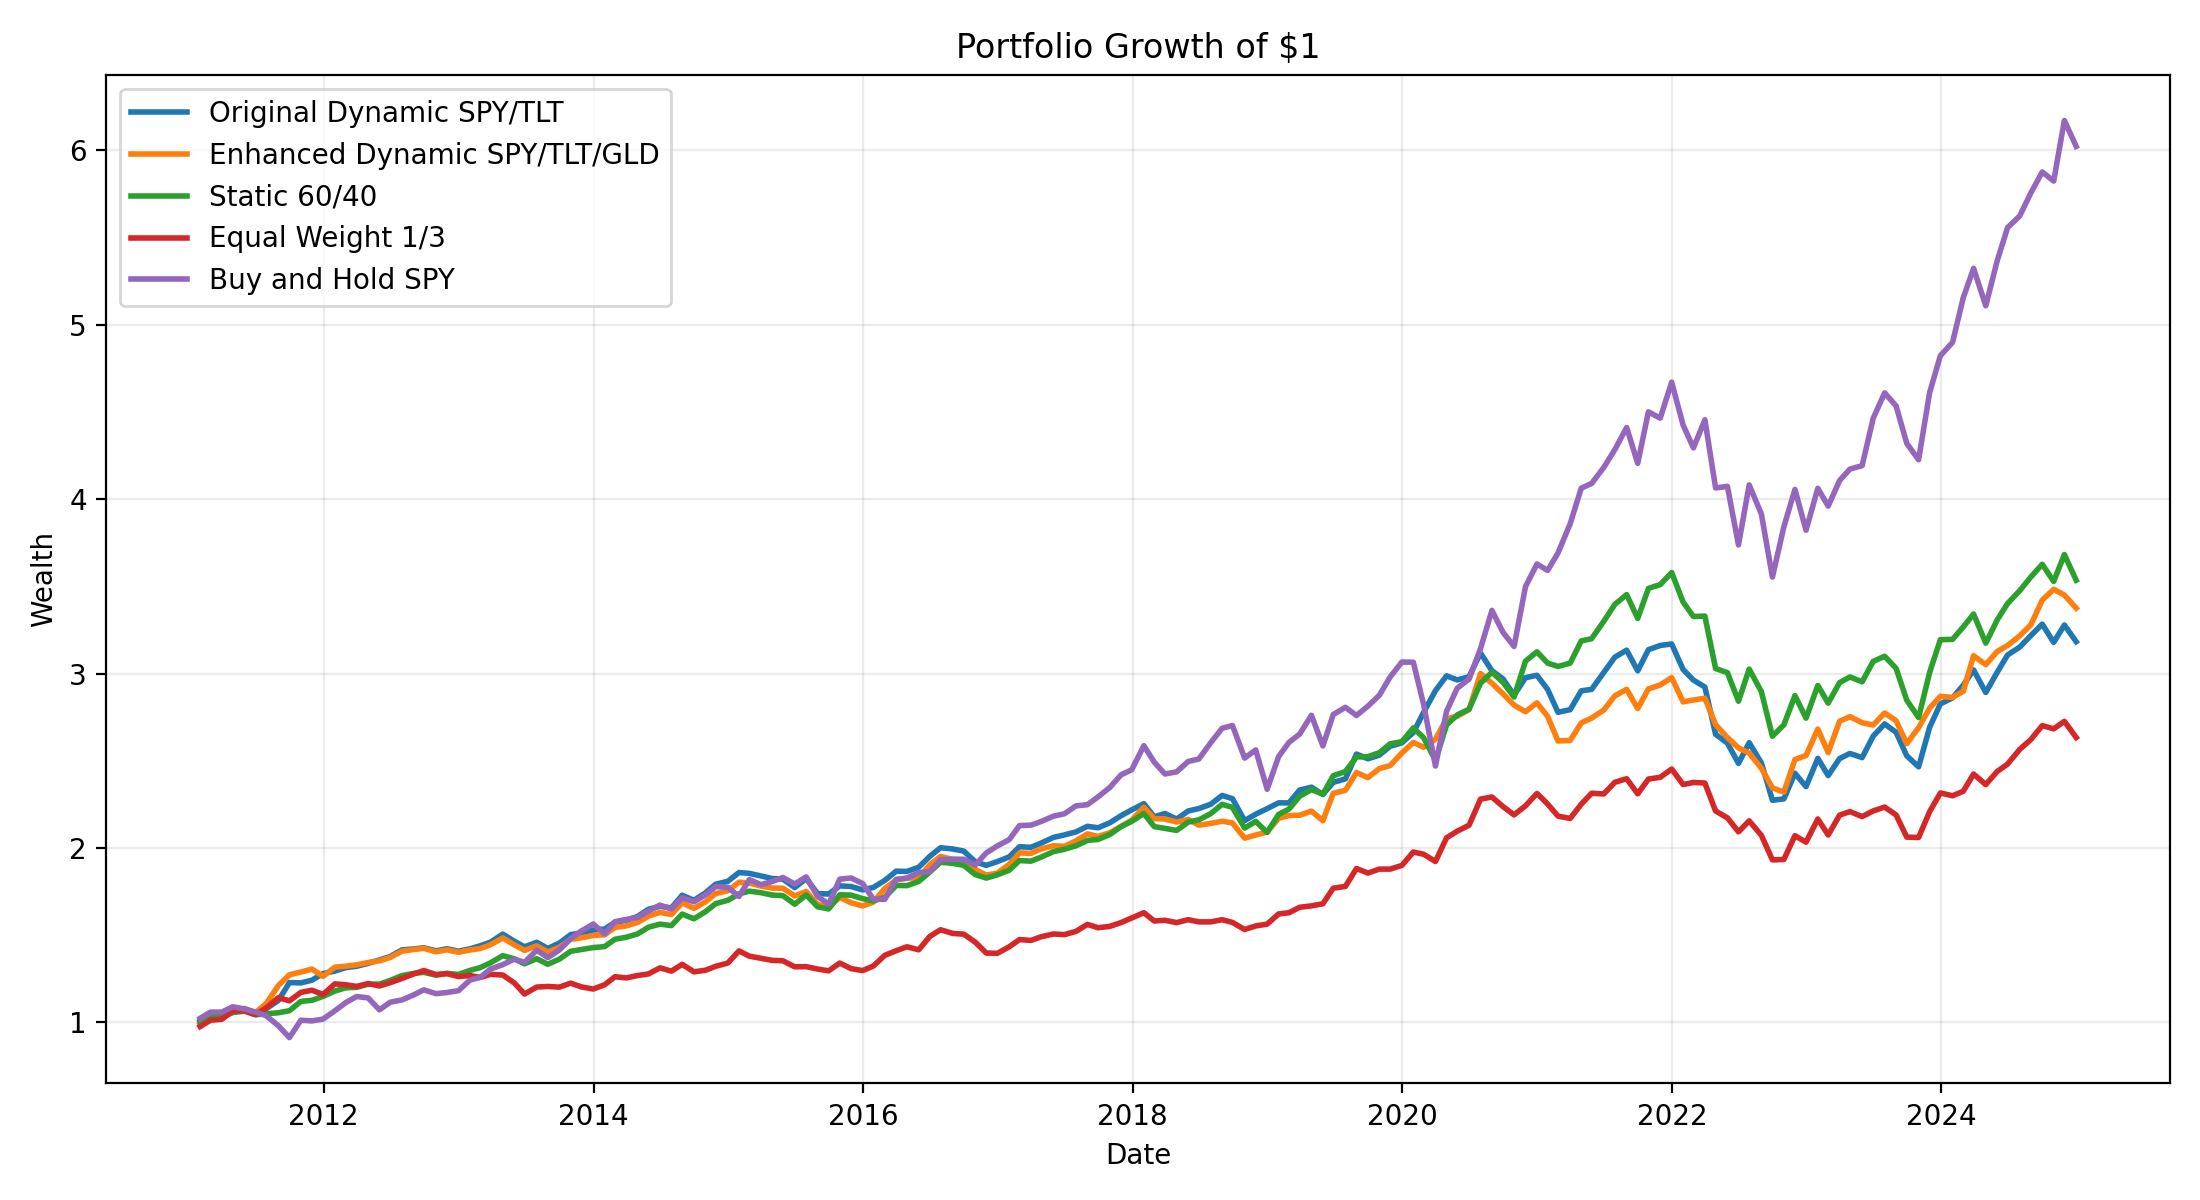
\includegraphics[width=\textwidth]{outputs/equity_curves.png}
\caption{Growth of \$1 across benchmark strategies}
\end{figure}

\begin{figure}[H]
\centering
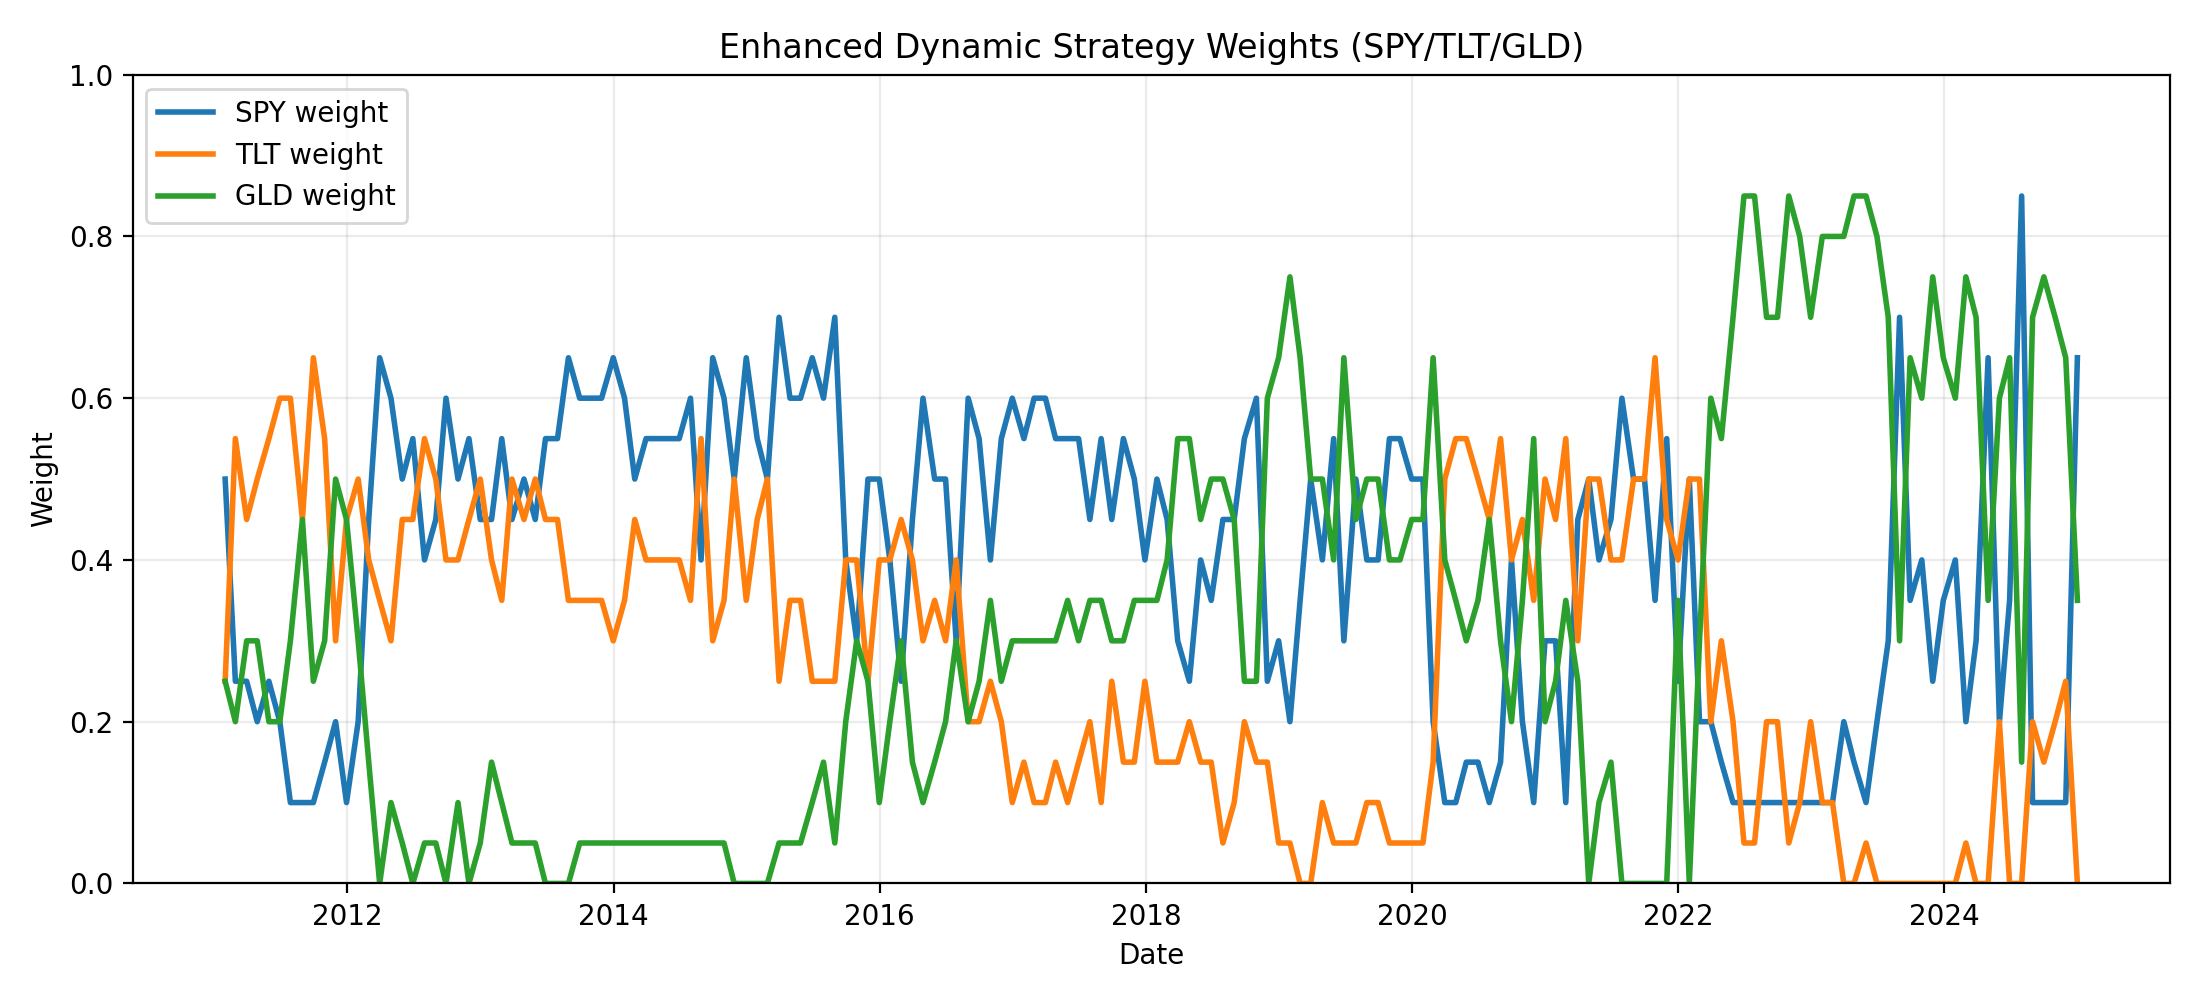
\includegraphics[width=\textwidth]{outputs/enhanced_dynamic_weights.png}
\caption{Enhanced strategy weights over time}
\end{figure}

\begin{figure}[H]
\centering
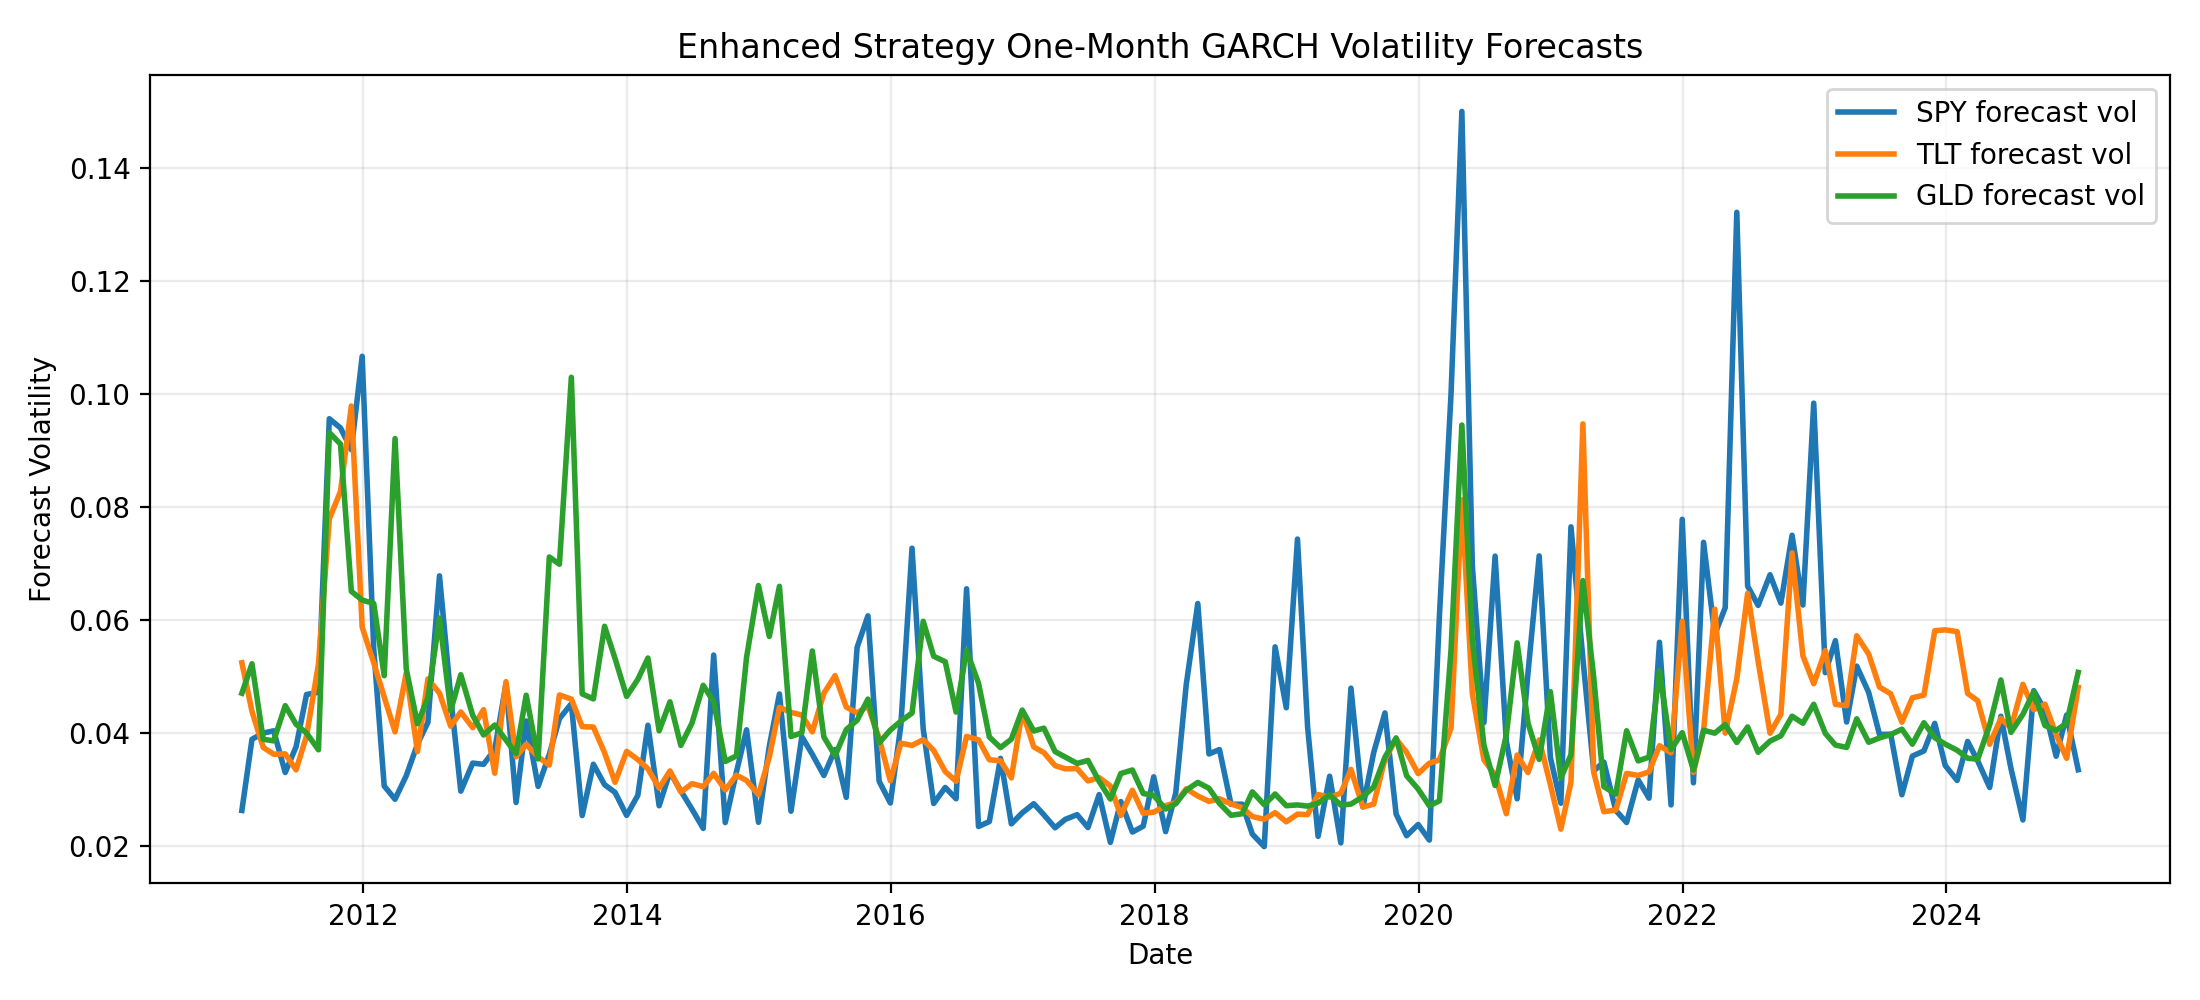
\includegraphics[width=\textwidth]{outputs/enhanced_forecast_volatility.png}
\caption{Enhanced strategy one-month GARCH volatility forecasts}
\end{figure}

\subsection{Interpretation}
There are three main takeaways.

First, the original proposal was directionally correct. Volatility forecasting plus CVaR-aware optimization does create a disciplined dynamic allocation process.

Second, the project became materially stronger once the asset universe was improved. This highlights a practical quant lesson: model quality depends not only on forecasting methods, but also on whether the portfolio opportunity set is well chosen.

Third, the final strategy is not the highest-return portfolio in absolute terms because buy-and-hold SPY benefits from strong equity compounding. However, the enhanced strategy delivers the best overall risk-adjusted performance and a much safer tail profile, which is exactly the point of a defensive allocator.

\section{Conclusion}
This final project started with a SPY/TLT volatility-managed CVaR allocation model and then improved it in a financially meaningful way by adding GLD as an alternative defensive sleeve. The resulting SPY/TLT/GLD strategy outperforms the original dynamic model on every major risk-adjusted metric and also exceeds the classic 60/40 benchmark in Sharpe ratio while lowering drawdown and tail risk.

The project therefore succeeds as a quantitative research study for two reasons:
\begin{itemize}
    \item it implements a clear and rigorous walk-forward backtest
    \item it produces a nontrivial research insight about portfolio construction under changing macro regimes
\end{itemize}

In short, the main lesson is that dynamic risk management works better when paired with a diversified defensive opportunity set. GARCH and CVaR help the allocator react to risk, but the addition of gold is what makes the strategy more robust when stock-bond diversification weakens.

\section{Limitations and Future Work}
\begin{itemize}
    \item The project still uses only three liquid ETFs, so the opportunity set remains small.
    \item GARCH is a simple volatility model and may miss richer nonlinear regime changes.
    \item Expected return estimates are based on momentum and can be noisy.
    \item The strategy is only tested on monthly rebalancing.
    \item Yahoo Finance data is convenient for research but not institutional-grade.
\end{itemize}

Future extensions include adding shorter-duration Treasury exposure such as IEF or SHY, using macro features for expected return estimation, introducing regime classification before optimization, and exploring reinforcement learning only after the state space and reward design are clearly defined.

\end{document}
